\section{Introduction}
\label{sec:introduction}

On-device intelligence is becoming a pipeline rather than a model.  A camera
frame may pass through a backbone and a task-specific head; an audio segment
passes through an encoder before decoding.  These stages exchange activations
that can exceed the original input, and their precedence couples resource
allocation: delay before publication leaves less slack for every downstream
stage.  Meanwhile, consolidating independent analytics is necessary to use an
expensive edge GPU efficiently.

MIG appears to provide the right substrate.  It isolates execution resources
and MIG-local allocations, and Jetson AGX Thor exposes fixed profiles suitable
for placing different stages~\cite{nvidiathormig}.  Its abstraction, however,
ends at each CUDA context.  A device allocation in one instance is not the
input object of another, and the hardware does not express that capacity
protected for a producer may be returned once its output becomes visible.
MPS can regulate active-thread shares inside an instance, but it does not
retract work already submitted by an independent client~\cite{nvidiamps}.
Consequently, isolation and quota control do not by themselves enforce a
pipeline deadline.

Existing serving abstractions inherit the same independent-client boundary.
GSLICE and gpulet tune spatial shares and placement for services
~\cite{gslice2020,gpulet2022}.  Kernel- and stream-level schedulers expose
finer control, but still need a first-class activation edge and an
arrival-to-completion contract to decide \emph{when} that control is safe.
The missing abstraction is therefore not another partition size.  It is the
lifecycle of a dependent request across isolated partitions.

\begin{figure*}[t]
  \centering
  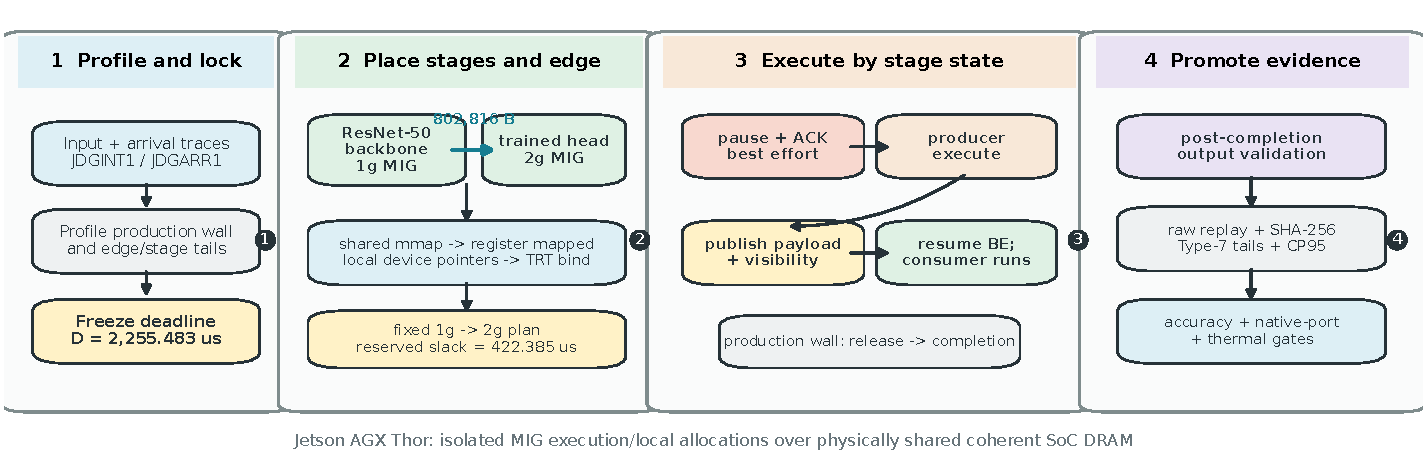
\includegraphics[width=\textwidth]{figures/p9-quiet-overview.pdf}
  \caption{The architecture and procedure of \sys.  The planner freezes a
  workload-specific deadline, places the two validated stages and their
  activation edge, and serializes the resulting contract.  At runtime,
  best-effort work is protected only through producer publication.  Accuracy,
  raw-replay, native-port, and thermal gates determine which results may be
  promoted.  The current production path is a two-stage chain, not a
  general-DAG runtime.}
  \Description{Four numbered modules show profiling and deadline locking,
  stage and activation-edge placement, publication-scoped execution, and
  evidence promotion on Jetson AGX Thor.}
  \label{fig:quiet-overview}
\end{figure*}

Jetson AGX Thor also supplies the key opportunity.  Although its MIG instances
isolate GPU execution and local allocation, the CPU and integrated GPU share
physical SoC DRAM.  A system-memory region can be mapped into separate
processes, registered in each selected CUDA context, and bound directly to
TensorRT I/O.  This preserves isolation while making the \emph{same physical
activation bytes} addressable by both stages.  The opportunity does not make
communication free: visibility, notification, shared-SoC contention, and
consumer queueing remain on the critical path.  A useful runtime must measure
these effects jointly and couple them to admission.

This observation raises our central question:
\begin{quote}
\emph{Can an edge runtime carry a real activation across isolated GPU
partitions, reclaim producer capacity, and still meet a frozen request
deadline?}
\end{quote}

We answer with \sys, whose procedure is shown in
Figure~\ref{fig:quiet-overview}.  \sys first profiles a concrete two-stage
TensorRT chain and freezes a deadline from independent calibration.  It then
selects the MIG UUIDs, quotas, edge transport, protection scope, and admission
state before creating GPU processes.  The data plane starts from a shared
\texttt{mmap}.  Each process invokes \texttt{cudaHostRegisterMapped}, then
obtains a local pointer with \texttt{cudaHostGetDevicePointer}.  TensorRT
binds that pointer directly.  We call this
path the \emph{full-coherent registered system-memory activation edge}.  It is
neither a CUDA managed-memory path nor a shared device allocation.

At runtime, an operational arrival trace releases each request independently
of the previous request's acknowledgement or validation.  \sys drains and
pauses the best-effort tenant, executes the producer, publishes the activation,
and immediately resumes the tenant while the consumer executes.  Checksums
and output capture occur after the production-completion boundary.  Thus, the
reported latency includes queueing and protection but excludes work performed
solely to validate the experiment.

NVIDIA MPS is our vendor baseline.  A native XSched path supplies the
fine-grained baseline~\cite{xsched2025}.  A separately scoped native Pantheon
gate~\cite{pantheon2024} uses a distinct integer-microsecond adapter contract
and is not pooled with the six-session table.  Orion~\cite{orion2024} remains
outside numeric claims because its upstream differential decision gate is
incomplete.  BLESS~\cite{bless2025} and independent-service provisioners
remain structural comparisons when their published mechanisms cannot execute
the identical dependency contract.
DeepPlan~\cite{deepplan2023} motivates direct host access, while edge runtimes
such as Miriam and Pantheon~\cite{miriam2023,pantheon2024} establish
complementary model-aware and preemptive designs.  We retain their names only
for faithful native mechanisms, never for a local approximation.

Our evaluation produces four results.  First, both a 90-request ImageNette
classification gate and a 10-request LibriSpeech ASR gate preserve their
reference metrics; the latter produces byte-identical output traces.  Second,
same-activation causal replay shows that precedence changes shared-resource
overlap, not merely copy time: across three exploratory pairs, \sys's
dependent execution has a $2{,}081.286~\mu$s lower mean p99 than the replayed
independent arm.  Third, in the thermal-normalized campaign, \sys is the only
tested system whose 95\% upper deadline-miss bound qualifies for the 0.05\%
target.  Fourth, offered-load points reveal the expected statistical boundary:
three 3,300-request points can describe behavior but cannot certify a
0.05\% target when zero misses alone would still yield a 0.0907\% upper bound.

\noindent\textbf{Contributions.}
\begin{enumerate}[leftmargin=*,itemsep=1pt,topsep=2pt]
  \item We identify \emph{dependency blindness} as a missing systems
  abstraction between isolated GPU partitions: placement must include the
  activation edge and protection must follow publication state.
  \item We implement a full-coherent registered system-memory activation edge
  for unmodified TensorRT engines in separate Thor MIG contexts, together with
  request-indexed activation replay and post-completion output validation.
  \item We design a hash-bound planner and stage-aware quiescence protocol that
  reserves a measured joint tail and resumes best-effort work immediately
  after producer publication.
  \item We provide two real-application semantic gates, two faithful
  published-system paths, request-level raw replay, exact deadline-miss
  confidence bounds, and six counterbalanced thermal sessions.
\end{enumerate}

The remainder of the paper describes the hardware and scheduling mismatch
(\S\ref{sec:background}), the \sys design (\S\ref{sec:design}) and
implementation (\S\ref{sec:implementation}), and the evidence and its explicit
promotion boundaries (\S\ref{sec:evaluation}).
